\newsavebox{\plotbox}
\sbox{\plotbox}{%
  \includegraphics[width=0.17\textwidth]{figures/restored/proposed_1}%
}
\newlength{\plottotalheight}
\setlength{\plottotalheight}{\dimexpr\ht\plotbox+\dp\plotbox\relax}
% 
\begin{figure*}[t]
    \begin{center}
        \begin{minipage}{0.95\textwidth}
            \centering
            \begin{minipage}[t]{0.17\textwidth}
                \centering
                \includegraphics[width=\linewidth]{figures/true_and_observed/true_signal}
            \end{minipage}\hspace{0.3em}
            \begin{minipage}[t]{0.17\textwidth}
                \centering
                \includegraphics[width=\linewidth]{figures/restored/glr}
            \end{minipage}\hspace{0.3em}
            \begin{minipage}[t]{0.17\textwidth}
                \centering
                \includegraphics[width=\linewidth]{figures/restored/gtv}
            \end{minipage}\hspace{0.3em}
            \begin{minipage}[t]{0.17\textwidth}
                \centering
                \includegraphics[width=\linewidth]{figures/restored/proposed_1}
            \end{minipage}\hspace{0.3em}
            \begin{minipage}[t]{0.17\textwidth}
                \centering
                \includegraphics[width=\linewidth]{figures/restored/proposed_2}
            \end{minipage}\hspace{2em}
            \begin{minipage}[t]{0.05\textwidth}
                \centering
                \makebox[0pt][l]{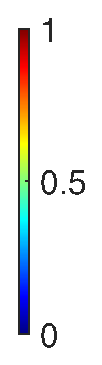
\includegraphics[totalheight=\plottotalheight, keepaspectratio]{figures/color_bar/jet}}
            \end{minipage}
        \end{minipage}
    \end{center}
    
    \begin{center}
        \begin{minipage}{0.95\textwidth}
            \centering
            \begin{minipage}[t]{0.17\textwidth}
                \centering
                \includegraphics[width=\linewidth]{figures/true_and_observed/observed_signal}
                \subcaption{\centering{True (upper) \\ observed (lower)}}
            \end{minipage}\hspace{0.3em}
            \begin{minipage}[t]{0.17\textwidth}
                \centering
                \includegraphics[width=\linewidth]{figures/residual_plot/glr}
                \subcaption{\centering{GLR \\ MSE = $0.0714$}}
            \end{minipage}\hspace{0.3em}
            \begin{minipage}[t]{0.17\textwidth}
                \centering
                \includegraphics[width=\linewidth]{figures/residual_plot/gtv}
                \subcaption{\centering{GTV \\ MSE = $0.0530$}}
            \end{minipage}\hspace{0.3em}
            \begin{minipage}[t]{0.17\textwidth}
                \centering
                \includegraphics[width=\linewidth]{figures/residual_plot/proposed_1}
                \subcaption{\centering{Ours (\ref{equation:proposed_1}) \\ MSE = $\underline{0.0387}$}}
            \end{minipage}\hspace{0.3em}
            \begin{minipage}[t]{0.17\textwidth}
                \centering
                \includegraphics[width=\linewidth]{figures/residual_plot/proposed_2}
                \subcaption{\centering{Ours (\ref{equation:proposed_2}) \\ MSE = $\mathbf{0.0364}$}}
            \end{minipage}\hspace{2em}
            \begin{minipage}[t]{0.05\textwidth}
                \centering
                \makebox[0pt][l]{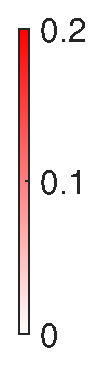
\includegraphics[totalheight=\plottotalheight,keepaspectratio]{figures/color_bar/red}}
            \end{minipage}
        \end{minipage}
    \end{center}
        
    \caption{Visual results and NMSEs in one run of noiseless inpainting, where the edges with corrupted weights are highlighted in thicker black.
             The first column shows the true signal (upper) and the observed signal (lower), with the masked signal elements as cross symbols. 
             In the remaining columns, the first row shows the recovered signals, and the second row highlights the error between the true and restored signals. 
             The proposed regularizations improved the recovery accuracy on nodes where GLR and GTV failed, demonstrating that they successfully inherited different strengths from GLR and GTV.}
    \label{visuals:qualitative_results}
\end{figure*}